\documentclass{article}
\usepackage{tikz}    % Fazer figuras
\usepackage{subcaption}

\begin{document}

\begin{figure}
    \centering
    \captionsetup[subfigure]{position=above}
    \begin{subfigure}[t]{0.45\textwidth}
    \centering
    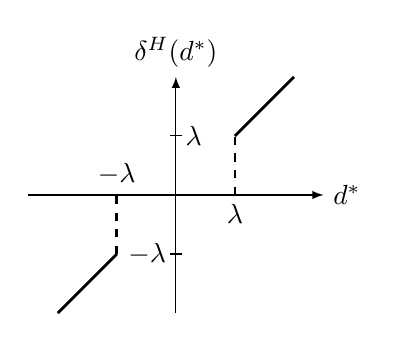
\begin{tikzpicture}[scale=0.75]
        % Eixos
        \draw[->, >=latex] (-2.5,0) -- (2.5,0) node[anchor=west] {$d^*$};
        \draw[->, >=latex] (0,-2) -- (0,2) node[anchor=south] {$\delta^H(d^*)$};
        
        % Gráfico
        \draw[line width = 1pt] (-2, -2) -- (-1,-1);
        \draw[line width = 1pt, dashed] (-1,-1) -- (-1, 0);
        \draw[line width = 1pt] (-1,0) -- (1, 0);
        \draw[line width = 1pt, dashed] (1,0) -- (1, 1);
        \draw[line width = 1pt] (1,1) -- (2, 2);
        
        % Pontos
        \node[anchor=south] at (-1,0) {$-\lambda$};
        \node[anchor=north] at (1,0) {$\lambda$};
        \draw (3pt,1) -- (-3pt, 1);
        \node[anchor=west] at (0,1) {$\lambda$};
        \draw (3pt,-1) -- (-3pt, -1);
        \node[anchor=east] at (0,-1) {$-\lambda$};
    \end{tikzpicture}
    \caption{Regra de limiar duro}
    \end{subfigure}
    \hspace{0.5cm}
    \begin{subfigure}[t]{0.45\textwidth}
    \centering
    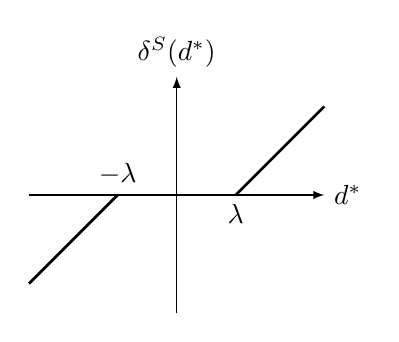
\begin{tikzpicture}[scale=0.75]
        % Eixos
        \draw[->, >=latex] (-2.5,0) -- (2.5,0) node[anchor=west] {$d^*$};
        \draw[->, >=latex] (0,-2) -- (0,2) node[anchor=south] {$\delta^S(d^*)$};
        
        % Gráfico
        \draw[line width = 1pt] (-2.5, -1.5) -- (-1,0);
        \draw[line width = 1pt] (-1,0) -- (1, 0);
        \draw[line width = 1pt] (1,0) -- (2.5, 1.5);
        
        % Pontos
        \node[anchor=south] at (-1,0) {$-\lambda$};
        \node[anchor=north] at (1,0) {$\lambda$};
    \end{tikzpicture}
    \caption{Regra de limiar suave}
    \end{subfigure}

    \caption{Regra de limiar duro e suave}
\end{figure}
\end{document}